% ============================================================================
% Accessibility
% ============================================================================
\DocumentMetadata{
  lang = en-US, 
  pdfstandard = ua-2, 
  tagging = on, 
  tagging-setup = {math/setup=mathml-SE}
}

% ============================================================================
% Document Properties - used on title slide and PDF metadata fields
% ============================================================================
\def\PresTitle{Managing Safety and Health Programs}     % Required - top line of title slide
\def\PresSubtitle{Baker College Engineering}            % Optional - second line
\def\PresAuthor{Brad Peirson}                           % Required - below dividing line
\def\PresInstitute{College of Information Technology and Engineering}       % Optional
\def\PresDate{}                                         % Optional
\def\PresKeywords{}                                     % Optional - used for hyperref

% Presentation Formatting
% ============================================================================
% ============================================================================
% Class Declaration
% ============================================================================
\documentclass[
        mode = handout,     % Projector = one bullet at a time, Handout = all
        font-size=14pt,     % Only accepts 9, 10, 12, 14, 17, 20
        pdfusetitle         % Pulls \title property from document
    ]
    {ltx-talk}              % ltx-talk class

% ============================================================================
% Custom Colors
% ============================================================================
\usepackage[table]{xcolor}
% Colors from the Baker College Style Guide
%\definecolor{BakerADARed}{RGB}{231, 0, 46}   % #e7002e Official ADA red-doesn't pass WCAG AAA for small text
\definecolor{BakerADARed}{RGB}{181, 0, 36}    % #b50024 Adjusted ADA red-passes WCAG AAA for small text
\definecolor{HoneyYellow}{RGB}{255, 196, 0}   % #ffc400
\definecolor{UpNorthGreen}{RGB}{114, 191, 68} % #72bf44
\definecolor{LakeBlue}{RGB}{134, 183, 227}    % #86b7e3
\definecolor{BakerADI}{RGB}{58, 98, 170}
\definecolor{BakerCIM}{RGB}{217, 35, 47}
\definecolor{BakerBlack}{RGB}{31, 34, 40}     % #1f2228
\definecolor{BakerWhite}{RGB}{255, 255, 255}
\definecolor{BakerRed}{RGB}{239, 0, 48}
\definecolor{Abbey}{RGB}{80, 82, 88}
\definecolor{RollingStone}{RGB}{121, 124, 126}
\definecolor{HitGray}{RGB}{165, 169, 172}
\definecolor{Iron1}{RGB}{201, 206, 209}
\definecolor{Iron}{RGB}{222, 225, 226}
\definecolor{BlackHaze1}{RGB}{237, 240, 240}
\definecolor{BlackHaze}{RGB}{245, 247, 247}

% ============================================================================
% Document Data
% ============================================================================
\title{\PresTitle}
\author{\PresAuthor}
\institute{\PresInstitute}
\date{\PresDate}

%Set up the hyperlink colors
\hypersetup{colorlinks,
    linkcolor=BakerBlack,
    urlcolor=BakerADARed,
    pdfauthor = {\PresAuthor},
    %pdftitle = {\PresentationTopic},   % Title is pulled directly
    pdfsubject = {\PresSubtitle},
    pdfkeywords = {\Keywords},
    pdfcreator = {LaTeX with hyperref package},
    pdfproducer = {LuaLaTeX}
    }

% Map your custom style guide colors to the progress bar aliases
\colorlet{pbcomplete}{BakerADARed}
\colorlet{pbincomplete}{Iron}

\usepackage[most]{tcolorbox}

% ============================================================================
% Footer Format
% ============================================================================
\EditInstance{footer}{std}{
  color         = Abbey,
  separator     = \hfill,
  element-order = {title, institute, framenumber},
  right-hspace  = 3mm,
  left-hspace   = 3mm,
}

% \DeclareInstance{footer}{empty}{
%   element-order = {}
% }

% ============================================================================
% Progress Bar Toggles & Helper Macros
% ============================================================================
\usepackage{xfp}        % Needed for floating point math
\newif\ifprogressbar    % Used to determine whether or not to show the bar
\progressbartrue        % Set the bar to true at the start

% Helper macro to automatically turn off the progress bar inside title/section frames
\newcommand{\makeblindframe}[1]{%
  \progressbarfalse
  #1%
  \progressbartrue
}

% ============================================================================
% Custom Page Formats
% ============================================================================
\let\oldmaketitle\maketitle         % Backup the original maketitle command
\let\oldsection\section             % Backup the original section command
\let\oldsubsection\subsection       % Backup the original subsection command

\makeatletter
\renewcommand{\maketitle}{%
\makeblindframe{%
  \disableglobalbackground
  \slidebackground{PresentationTitleGraphic_2048x1151}%
  \color{white}%
  %\UseInstance{footer}{wallpaper}
  \begin{frame}[wallpaper]
    \vspace*{1in}%
      \begin{tcolorbox}[
          enhanced,
          colback=black,       
          colframe=black,      
          opacityfill=0.25,       
          arc=6pt,                
          boxrule=0pt,            
          left=20pt, right=20pt,  
          top=20pt, bottom=20pt,
          width=0.90\textwidth,   
          halign=left             
      ]
          \color{white}%
          % Title (Always visible)
          {\large\bfseries\sffamily \@title}\\[0.5em]%
          
          % Conditional Subtitle
          \ifx\PresSubtitle\empty
          \else
            {\normalsize\sffamily \PresSubtitle}\\[0.5em]%
          \fi
          
          % High-contrast divider line
          {\color{white!80}\rule{0.3\textwidth}{0.8pt}}\\[0.5em]%
          
          % Author (Always visible)
          {\small\sffamily \@author}\\%
          
          % Conditional Institute
          \ifx\PresInstitute\empty
          \else
            {\small\sffamily \PresInstitute}\\%
          \fi
          
          % Conditional Date
          \ifx\PresDate\empty
          \else
            {\small\sffamily \@date}\\%
          \fi
      \end{tcolorbox}%
      \vfill     
  \end{frame}%
  \enableglobalbackground{BG}%
  \color{black}%
  %\UseInstance{footer}{std}
}%
}
\makeatother

% Create a variable container to hold the current section title
\newcommand{\currentsectiontitle}{}

% Redefine \section to take 1 argument (the title)
\renewcommand{\section}[1]{%
\makeblindframe{%
  \renewcommand{\currentsectiontitle}{#1}%
  \disableglobalbackground
  \slidebackground{PresentationSectionBackground_2048x1151}%
  \begin{frame}
    \vfill
    %\vspace*{0.625in}%
    \begin{tcolorbox}[
        enhanced,
        colback=black,       
        colframe=black,      
        opacityfill=0.25,       
        arc=6pt,                
        boxrule=0pt,            
        left=20pt, right=20pt,  
        top=20pt, bottom=20pt,
        width=0.80\textwidth,   
        halign=left             
    ]
        \color{white}%
        {\large\bfseries\sffamily #1}\\[0.5em]%   
    \end{tcolorbox}%
    \vfill 
  \end{frame}%
  \oldsection{#1}%
  \enableglobalbackground{BG}%

  % This will be used for an auto TOC at every section
  % Right now ltx-talk TOC is still in development
  % Once it comes a little further along this can be used
  % \begin{frame}
  %       \frametitle{Section Overview}
  %       \tableofcontents[sections=\thesection]
  %   \end{frame}%
}%
}

% Redefine \subsection to take 1 argument
\renewcommand{\subsection}[1]{%
\makeblindframe{%
  \disableglobalbackground
  \slidebackground{PresentationSectionBackground_2048x1151}%
  \begin{frame}
    \vfill
    %\vspace*{0.25in}% 
    \begin{tcolorbox}[
        enhanced,
        colback=black,       
        colframe=black,      
        opacityfill=0.25,       
        arc=6pt,                
        boxrule=0pt,            
        left=20pt, right=20pt,  
        top=20pt, bottom=20pt,
        width=0.80\textwidth,   
        halign=left             
    ]
        \color{white}%
        {\large\bfseries\sffamily\currentsectiontitle}\\[0.5em]%
        {\normalsize\sffamily #1}%
    \end{tcolorbox}%
    \vfill 
  \end{frame}%
  \oldsubsection{#1}%
  \enableglobalbackground{BG}%
}%
}

%Set the fonts to use NeueHaas Grotesk
\setsansfont{NHAASGROTESKTXPRO-}[
    Path=../NeueHaasGroteskFiles/,
    Scale=1.0,
    Extension = .ttf,
    UprightFont=*55Rg,
    BoldFont=*75Bd,
    ItalicFont=*56It,
    BoldItalicFont=*76BdIt
    ]

% Force the document default family to Sans-Serif
\renewcommand{\familydefault}{\sfdefault}

\usepackage{mathtools} % Load BEFORE unicode math settings
\setmathfont{Fira Math}[Scale=MatchLowercase] 

% 1. Turn global background ON
\newcommand{\enableglobalbackground}[1]{%
  \AddToHook{shipout/background}[mybg]{%
    \put(0, -\paperheight){%
      \includegraphics[width=\paperwidth, height=\paperheight, artifact]{#1}%
    }%
  }%
}

% 2. Turn global background OFF
\newcommand{\disableglobalbackground}{%
  \RemoveFromHook{shipout/background}[mybg]%
}

\newcommand{\slidebackground}[1]{%
  \AddToHookNext{shipout/background}{%
    \put(0, -\paperheight){%
      \includegraphics[width=\paperwidth, height=\paperheight, artifact]{#1}%
    }%
  }%
}

% --- GLOBAL BULLET OVERRIDES ---
\renewcommand{\labelitemi}{\color{BakerBlack}\Large\textbullet}
\renewcommand{\labelitemii}{\color{BakerBlack}\large\textbullet}
\renewcommand{\labelenumi}{\color{BakerBlack}\bfseries\arabic{enumi}.}
\renewcommand{\labelenumii}{\color{BakerBlack}\bfseries\alph{enumii})}

\AddToHook{begindocument/before}{%
  \EditInstance{item}{description}{
    label-format = \normalfont\bfseries\color{BakerADARed}#1
  }%
}

\AddToHook{begindocument/before}{%
  \EditInstance{item}{basic}{
    label-format = \color{BakerADARed}#1
  }%
}

% Global override for ltx-talk slide titles
\EditInstance{frametitle}{header}{
    font = \rule{0pt}{1.5cm}\bfseries\Large,
}

\EditInstance{header}{std}{
    font = \bfseries\huge,
    color = BakerBlack,
}

\AddToHook{env/block/begin}{%
  \colorlet{structure}{BakerADARed}%
}

\pretocmd{\tableofcontents}{\begin{minipage}{\textwidth} \linespread{1.4}}{}{}
\apptocmd{\tableofcontents}{\end{minipage}}{}{}

%Biber not functional in ltx-talk as of 2026-05-29
%Package that allows the creation of bibliographies
\usepackage[
    backend=biber,
    style=authoryear,
    sorting=none,
    %entryhead=false
    ]{biblatex}

%Load the bibliography file
\addbibresource{../../reference.bib}

\defbibheading{bibslide}{References}

\newcolumntype{L}[1]{>{\raggedright\let\newline\\\arraybackslash\hspace{0pt}}m{#1}}
\newcolumntype{C}[1]{>{\centering\let\newline\\\arraybackslash\hspace{0pt}}m{#1}}
\newcolumntype{R}[1]{>{\raggedleft\let\newline\\\arraybackslash\hspace{0pt}}m{#1}}

%All of the graphics are in a seperate folder, this makes it so the folder doesn't have to be repeated every time
\graphicspath{
  {../assets/images}
  {../assets/diagrams}
  {../assets/plots}
}

\makeatletter
% New counter to hold the custom "max frames" for the progress bar
\newcommand{\pb@maxtotal}{1}

% Read the custom total from the .aux file if it exists
\AtBeginDocument{%
  \ifdefined\pb@storedtotal
    \let\pb@maxtotal\pb@storedtotal
  \else
    % Fallback to standard total if our custom hook hasn't run yet
    \edef\pb@maxtotal{\@totalframes}%
  \fi
}

% Custom Appendix command that caps the progress bar and turns it off
\newcommand{\talkappendix}{%
  % 1. Write the CURRENT frame number to the .aux file as the progress total
  \immediate\write\@auxout{\string\gdef\string\pb@storedtotal{\@framenumber}}%
  % 2. Turn off the progress bar for all subsequent appendix slides
  \progressbarfalse
}
\makeatother

% ============================================================================
% Progress Bar Logic 
% ============================================================================
\makeatletter               
\AddToHook{shipout/background}{%
  \ifprogressbar
    % Read ltx-talk's internal frame counter safely
    \edef\currentframe{\@framenumber}%
    \edef\totalframes{\pb@maxtotal}% Use our custom max total instead
    
    % Fallback checks: If the document hasn't fully compiled yet, default to 1
    \ifx\currentframe\empty\def\currentframe{1}\fi
    \ifx\totalframes\empty\def\totalframes{1}\fi
    
    % Draw the progress bar if we have a valid total frame count
    \ifnum\totalframes>1\relax
      % Compute fraction width: (current - 1) / (total - 1)
      \edef\pbfraction{\fpeval{(\currentframe - 1) / (\totalframes - 1)}}%
      
      % Guard rails to prevent the bar from overshooting 100% on a first compile
      \ifdim\pbfraction pt>1pt\def\pbfraction{1}\fi 
      
      \edef\completewidth{\fpeval{\pbfraction * \paperwidth}}%
      \edef\incompletewidth{\fpeval{\paperwidth - \completewidth}}%
      
      % Render full-width progress bar at the top edge
      \put(0cm, -0.1cm){%
        \color{pbcomplete}\rule{\completewidth pt}{2pt}%
        \color{pbincomplete}\rule{\incompletewidth pt}{2pt}%
      }%
    \fi
  \fi
}
\makeatother

% 1. Globally shrink all caption components right as the caption engine fires
\AddToHook{cmd/@makecaption/before}{\footnotesize}

% 2. Declare and assign a blank plug to the kernel's caption label socket
\NewSocketPlug{caption/label}{nolabel}{}
\AssignSocketPlug{caption/label}{nolabel}

\usepackage{adjustbox}

\usepackage{amssymb}
\usepackage{amsmath}

\usepackage{animate}

\usepackage{calc} % Optional, but helpful for layout

\usepackage{multirow}

\usepackage[americanvoltages]{circuitikz}
\usepackage{pgfplots}
\usepackage{pgf-pie}

\usetikzlibrary{
    intersections, 
    fillbetween,
    patterns,
    decorations.pathreplacing,
    decorations.pathmorphing,
    decorations.text,
    decorations.markings,
    arrows.meta,
    arrows,
    shapes,
    shapes.geometric,
    shadows,
    calligraphy,
    backgrounds,
    intersections,
    calc,
    math,
    positioning,
    svg.path,
    shadows,
    shadows.blur,
    shadings
    }

\pgfplotsset{compat=1.18}

\pgfdeclarelayer{ft}
\pgfdeclarelayer{bg}
\pgfsetlayers{bg, main, ft}

% Usage: \hexpic[]{height}{Alt text}{Attribution}{image path}
\newcommand{\hexpic}[5][]{%
  \begin{figure}
    \centering
    \begin{tikzpicture}[
      baseline=(hex.base),      
      every shadow/.style={
        shadow opacity=70
        }
      ]
      \node (hex) [
        draw=white, 
        minimum size=#2, 
        regular polygon, 
        regular polygon sides=6, 
        rotate=90,
        blur shadow
      ] {};
      \begin{scope}
        \clip (hex.corner 1) -- (hex.corner 2) -- (hex.corner 3) -- 
              (hex.corner 4) -- (hex.corner 5) -- (hex.corner 6) -- cycle;
        \node at (hex.center) [#1] {
          \includegraphics[height=#2, alt={#3}]{#5}
        };
      \end{scope}
    \end{tikzpicture}

    \vspace{0.5em}
    {\tiny #4\par}
  \end{figure}  
}

% Usage: \shadowpic[]{width}{Alt text}{Attribution}{image path}
\newcommand{\shadowpic}[5][]{%
  \begin{figure}
    \centering
    \begin{tikzpicture}
      [every shadow/.style={
        shadow opacity=70
        }
      ]
      \node (image) [
        inner sep=0,
        blur shadow
      ] {\includegraphics[width=#2, alt={#3}]{#5}};
    \end{tikzpicture}

    \vspace{0.5em}
    {\tiny #4\par}
  \end{figure}
}

\tikzset{middlearrow/.style={
        decoration={markings, 
        mark= at position 0.5 with {\arrow{#1}},
        },
        postaction={decorate}
    }
}

% Usage: \tikztodo[width]{height}{description/notes}
\newcommand{\tikztodo}[3][0.8\textwidth]{%
  \begin{center}
    \fbox{%
      \parbox[c][#2][c]{#1}{%
        \centering
        \textbf{\textcolor{red}{TODO: TikZ Diagram}}\\[0.5em]
        \small #3%
      }%
    }%
  \end{center}%
}

% Macro: \drawrails{<number_of_1cm_segments>}
\newcommand{\drawrails}[1]{
  % Calculate total depth: 1 cm per segment
  \pgfmathsetmacro{\railheight}{-1 * #1}
  
  % L1 Rail (x = 0)
  \draw[thick] (0, 0) -- (0, \railheight cm);
    
  % L2 Rail (x = 15)
  \draw[thick] (15, 0) -- (15, \railheight cm);
}

\newcommand{\ccwplus}{%
  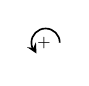
\begin{tikzpicture}[baseline=(char.base)]
    \node(char) at (0,0) {\(\scriptscriptstyle +\)};
    \draw[->, >=stealth, semithick] (0.2,0) arc (0:230:0.18cm);
  \end{tikzpicture}%
}

%====================================================================================
% Timer Ladder Symbol - Could be used for TON, TOF, RTO....
%====================================================================================
\tikzset{
    TON/.pic={

        \draw[
          BakerBlack
        ]
        (0,0)
        -- ++(0,0.375)
        -- ++(3.5,0)
        coordinate[pos=0.5](-TOP)
        -- ++(0,-1.75)
        coordinate[pos=3/14](-OUT)
        coordinate[pos=0.5](-EN1)
        coordinate[pos=0.875](-DN1)
        -- ++(-3.5,0)        
        -- (0,0)
        coordinate(-IN);

        \node[
          text=BakerBlack,
          font=\bfseries,
          anchor=east
        ](pre)
        at ($(-TOP)-(0,1.75em)$)
        {{\small PRE:}};

        \node[
          text=BakerBlack,
          font=\bfseries,
          anchor=east
        ](acc)
        at ($(pre.east)-(0,1em)$)
        {{\small ACC:}};

        \coordinate (-PRE) at (pre.east); % For the preset value
        \coordinate (-ACC) at (acc.east);

        \draw[
            BakerBlack
        ]
        (-EN1)
        -- ++(0.5,0)
        coordinate(-EN2)
        node[
            text=BakerBlack,
            anchor=west
        ]
        {{\small EN}};

        \draw[
            BakerBlack
        ]
        (-DN1)
        -- ++(0.5,0)
        coordinate(-DN2)
        node[
            text=BakerBlack,
            anchor=west
        ]
        {{\small DN}};

    }
}

%====================================================================================
% Oval ladder symbol, good for ONS, RES, etc.
%====================================================================================
\tikzset{
    ONS/.pic={

        \draw[
          BakerBlack
        ]
        (0,0)
        coordinate(-IN)
        -- ++(0.75,0)
        node[
          draw=BakerBlack, 
          text=BakerBlack, 
          font=\small, 
          minimum width=1.5cm, 
          minimum height=0.75cm, 
          anchor=west, 
          rounded corners=0.25cm
          ](ons){};
        
        \draw[BakerBlack] (ons.east) -- ++(0.75,0) coordinate(-OUT);

        \coordinate(-INS) at (ons.center);
        \coordinate(-VAR) at (ons.north); 
    }
}

%====================================================================================
% Source A, Source B, Dest box
%====================================================================================
\tikzset{
    SrcDest/.pic={
      
        \draw[
          BakerBlack
        ]
        (0,0)
        coordinate(-IN)
        -- ++(0,0.375)
        -- ++(5,0)
        coordinate[pos=0.5](-TOP)
        -- ++(0,-3.25)
        coordinate[pos=3/26](-OUT)
        -- ++(-5,0)
        -- (0,0)
        coordinate(l1);

        \node[
          text=BakerBlack,
          font=\bfseries,
          anchor=west
        ](srcA)
        at (l1)
        {{\small Src A:}};

        \node[
          text=BakerBlack,
          font=\bfseries,
          anchor=west
        ](srcB)
        at ($(l1)-(0,2em)$)
        {{\small Src B:}};

        \node[
          text=BakerBlack,
          font=\bfseries,
          anchor=west
        ](dest)
        at ($(srcB.west)-(0,2em)$)
        {{\small Dest:}};

        \coordinate(-SRCA) at (srcA.east);
        \coordinate(-AVAL) at ($(srcA.east)-(0,1em)$);
        \coordinate(-SRCB) at (srcB.east);
        \coordinate(-BVAL) at ($(srcB.east)-(0,1em)$);
        \coordinate(-DEST) at ($(-BVAL)-(0,1em)$);
        \coordinate(-DVAL) at ($(-DEST)-(0,1em)$);
    }
}

%====================================================================================
% Source A, Source B box
%====================================================================================
\tikzset{
    SrcAB/.pic={
      
        \draw[
          BakerBlack
        ]
        (0,0)
        coordinate(-IN)
        -- ++(0,0.375)
        -- ++(4,0)
        coordinate[pos=0.5](-TOP)
        -- ++(0,-2.25)
        coordinate[pos=1/6](-OUT)
        -- ++(-4,0)
        -- (0,0)
        coordinate(l1);

        \node[
          text=BakerBlack,
          font=\bfseries,
          anchor=west
        ](srcA)
        at (l1)
        {{\small Src A:}};

        \node[
          text=BakerBlack,
          font=\bfseries,
          anchor=west
        ](srcB)
        at ($(l1)-(0,2em)$)
        {{\small Src B:}};

        \coordinate(-SRCA) at (srcA.east);
        \coordinate(-AVAL) at ($(srcA.east)-(0,1em)$);
        \coordinate(-SRCB) at (srcB.east);
        \coordinate(-BVAL) at ($(srcB.east)-(0,1em)$);
    }
}

%====================================================================================
% LIMIT instruction
%====================================================================================
\tikzset{
    Limit/.pic={
      
        \draw[
          BakerBlack
        ]
        (0,0)
        coordinate(-IN)
        -- ++(0,0.375)
        -- ++(4,0)
        coordinate[pos=0.5](-TOP)
        -- ++(0,-3.25)
        coordinate[pos=3/26](-OUT)
        -- ++(-4,0)
        -- (0,0)
        coordinate(l1);

        \node[
          text=BakerBlack,
          font=\bfseries,
          anchor=west
        ](srcA)
        at (l1)
        {{\small Low:}};

        \node[
          text=BakerBlack,
          font=\bfseries,
          anchor=west
        ](srcB)
        at ($(l1)-(0,2em)$)
        {{\small Test:}};

        \node[
          text=BakerBlack,
          font=\bfseries,
          anchor=west
        ](dest)
        at ($(srcB.west)-(0,2em)$)
        {{\small High:}};

        \coordinate(-LO) at (srcA.east);
        \coordinate(-LOV) at ($(srcA.east)-(0,1em)$);
        \coordinate(-TEST) at (srcB.east);
        \coordinate(-TESTV) at ($(srcB.east)-(0,1em)$);
        \coordinate(-HI) at ($(-TESTV)-(0,1em)$);
        \coordinate(-HIV) at ($(-HI)-(0,1em)$);
    }
}

%====================================================================================
% Source Destination box
%====================================================================================
\tikzset{
    SrcSingle/.pic={
      
        \draw[
          BakerBlack
        ]
        (0,0)
        coordinate(-IN)
        -- ++(0,0.375)
        -- ++(6,0)
        coordinate[pos=0.5](-TOP)
        -- ++(0,-2.25)
        coordinate[pos=1/6](-OUT)
        -- ++(-6,0)
        -- (0,0)
        coordinate(l1);

        \node[
          text=BakerBlack,
          font=\bfseries,
          anchor=west
        ](srcA)
        at (l1)
        {{\small Source:}};

        \node[
          text=BakerBlack,
          font=\bfseries,
          anchor=east
        ](srcB)
        at ($(srcA.east)-(0,2em)$)
        {{\small Dest:}};

        \coordinate(-SRC) at (srcA.east);
        \coordinate(-SRCV) at ($(srcA.east)-(0,1em)$);
        \coordinate(-DEST) at (srcB.east);
        \coordinate(-DESTV) at ($(srcB.east)-(0,1em)$);
    }
}

%====================================================================================
% Compute Box
%====================================================================================
\tikzset{
    CPT/.pic={
      
        \draw[
          BakerBlack
        ]
        (0,0)
        coordinate(-IN)
        -- ++(0,0.375)
        -- ++(8.5,0)
        coordinate[pos=0.5](-TOP)
        -- ++(0,-1.75)
        coordinate[pos=3/14](-OUT)
        -- ++(-8.5,0)
        -- (0,0)
        coordinate(l1);

        \node[
          text=BakerBlack,
          font=\bfseries,
          anchor=west
        ](srcA)
        at (l1)
        {{\small Source:}};

        \node[
          text=BakerBlack,
          font=\bfseries,
          anchor=east
        ](srcB)
        at ($(srcA.east)-(0,2em)$)
        {{\small Exp:}};

        \coordinate(-DEST) at (srcA.east);
        \coordinate(-DESTV) at ($(srcA.east)-(0,1em)$);
        \coordinate(-EXP) at (srcB.east);
        \coordinate(-EXPV) at ($(srcB.east)-(0,1em)$);
    }
}

% ============================================================================
% Document Content
% ============================================================================
\begin{document}

\maketitle              % Redefined in the preamble to generate a full frame

\begin{frame}
    \frametitle{Agenda}
    \begingroup
        % Tighten the spacing between paragraphs/TOC lines
        \setlength{\parskip}{0.3em} 
        
        % Optionally tighten the line spacing within an entry
        %\baselineskip=1.2em 
        
        \setcounter{tocdepth}{1} % Show only sections
    \tableofcontents
    \setcounter{tocdepth}{2} % Reset back to default so subsections are tracked
    \endgroup
\end{frame}

\begin{frame}
    \frametitle{Objectives}
    \begin{enumerate}[<+- | alert@+>]
        \item Recognize the cost of workplace accidents
        \item Recognize the benefits of implementing an effective safety and health program
        \item Describe the elements of an effective safety and health program
        \item Identify three methods to prevent workplace hazards
    \end{enumerate}
\end{frame}

% \begin{frame}
%     \frametitle{Opening Video}
%     \begin{center}
%         \href{https://www.yout-ube.com/watch?v=k84-iy5yTFE}{OSHA FAIL 2020 | Compilation of funny workplace fail videos \cite{WorkplaceFails}}

%         \scriptsize{\href{https://www.yout-ube.com/watch?v=k84-iy5yTFE}{https://www.yout-ube.com/watch?v=k84-iy5yTFE}}
%     \end{center}    
% \end{frame}

\section{Introduction}

% Old data from OSHA presentation - 2015
% \begin{frame}
%     \frametitle{Fatal Occupation Injuries}

%     \shadowpic[]{0.5\linewidth}{Horizontal bar chart titled "Fatal occupational injuries by major event, 2015" showing a total of 4,836 fatal work injuries. The major event categories from top to bottom are: Transportation incidents (2,054 total, breakdown showing Roadway incidents at 1,264 and remaining at 790), Falls, slips, trips (800 total, breakdown showing Falls to lower level at 648 and remaining at 152), Contact with objects and equipment (722), Violence and other injuries by persons or animals (703 total, breakdown showing Homicides at 417 and remaining at 286), Exposure to harmful substances or environments (424), and Fires and explosions (121). A note at the bottom highlights that more fatal work injuries resulted from transportation incidents than any other event in 2015, with roadway incidents alone accounting for about one out of every four fatal work injuries. Source: U.S. Bureau of Labor Statistics, 2016.}{\textbf{Image:} U.S. Occupational Safety and Health Administration (OSHA)}{FatalInjuries}
% \end{frame}

\begin{frame}
    \frametitle{Fatal Occupational Injuries}

    \begin{figure}
        \centering
        \resizebox{0.75\linewidth}{!}{
            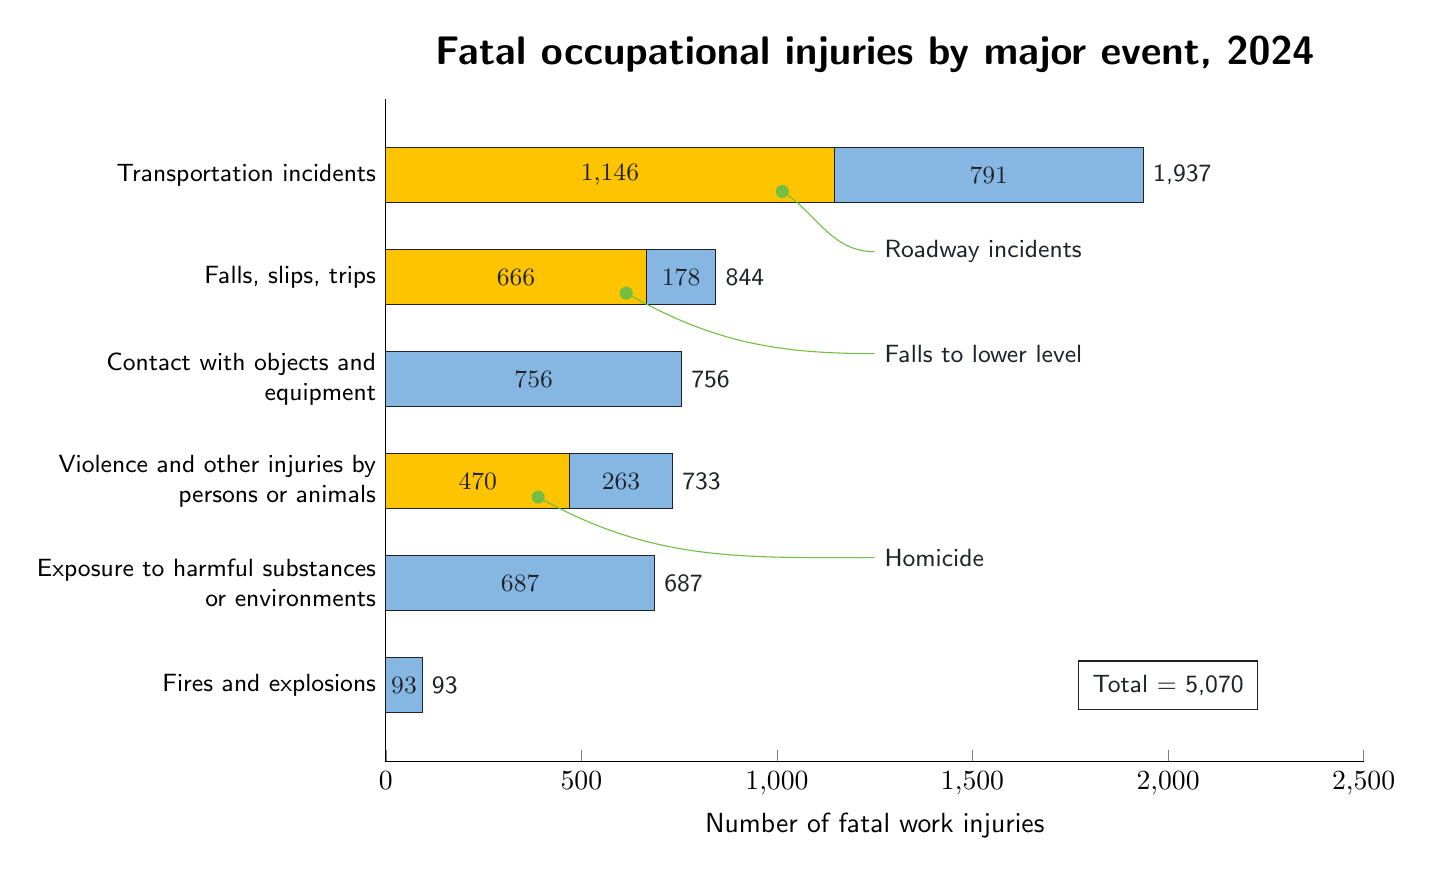
\begin{tikzpicture}
    \begin{axis}[
        xbar stacked,
        width=14cm,
        height=10cm,
        title={\textbf{\Large Fatal occupational injuries by major event, 2024}},
        xlabel={Number of fatal work injuries},
        xmin=0, xmax=2500,
        xtick={0, 500, 1000, 1500, 2000, 2500},
        ytick=data,
        yticklabels={
            {Fires and explosions},
            {Exposure to harmful substances\\or environments},
            {Violence and other injuries by\\persons or animals},
            {Contact with objects and\\equipment},
            {Falls, slips, trips},
            {Transportation incidents}
        },
        yticklabel style={
            % text width=5.5cm, 
            align=right, 
            font=\small
            },
        nodes near coords,
        nodes near coords style={font=\small, color=BakerBlack},
        bar width=20pt,
        enlarge y limits=0.15,
        legend style={at={(0.5,-0.15)}, anchor=north, legend columns=-1, draw=none},
        axis lines*=left,
        %x line yshift=-5pt,
    ]

        % Primary Sub-category (Darker Blue)
        \addplot[fill=HoneyYellow, draw=BakerBlack,] coordinates {
            (0,1)    % Fires and explosions (no sub-category)
            (0,2)    % Exposure to harmful substances
            (470,3)  % Homicides
            (0,4)    % Contact with objects
            (666,5)  % Falls to lower level
            (1146,6) % Roadway incidents
        };

        % Remaining Category Count (Lighter Blue)
        \addplot[fill=LakeBlue, draw=BakerBlack,] coordinates {
            (93,1)   % Fires and explosions (total = 93)
            (687,2)  % Exposure (total = 687)
            (263,3)  % Violence remaining (733 - 470 = 263)
            (756,4)  % Contact with objects (total = 756)
            (178,5)  % Falls remaining (844 - 666 = 178)
            (791,6)  % Transportation remaining (1937 - 1146 = 791)
        };

        \node[
            anchor=west,
            align=left,
            text=BakerBlack,
        ]
        at(1937,6)
        {\small{1,937}};

        \node[
            anchor=west,
            align=left,
            text=BakerBlack,
        ]
        at(844,5)
        {\small{844}};

        \node[
            anchor=west,
            align=left,
            text=BakerBlack,
        ]
        at(756,4)
        {\small{756}};

        \node[
            anchor=west,
            align=left,
            text=BakerBlack,
        ]
        at(733,3)
        {\small{733}};

        \node[
            anchor=west,
            align=left,
            text=BakerBlack,
        ]
        at(687,2)
        {\small{687}};

        \node[
            anchor=west,
            align=left,
            text=BakerBlack,
        ]
        at(93,1)
        {\small{93}};

            % Draw annotations on top after the axis finishes rendering:
        \pgfplotsset{
            after end axis/.code={
                \draw[UpNorthGreen, *-]
                    (axis cs:1000, 5.875) to[out=330,in=180] (axis cs:1250, 5.25)
                    node[anchor=west, text=BakerBlack] {{\small Roadway incidents}};

                \draw[UpNorthGreen, *-]
                    (axis cs:600, 4.875) to[out=330,in=180] (axis cs:1250, 4.25)
                    node[anchor=west, text=BakerBlack] {{\small Falls to lower level}};

                \draw[UpNorthGreen, *-]
                    (axis cs:375, 2.875) to[out=330,in=180] (axis cs:1250, 2.25)
                    node[anchor=west, text=BakerBlack] {{\small Homicide}};
                
                % Total box annotation
                \node[draw=BakerBlack, text=BakerBlack, inner sep=5pt, font=\small] at (axis cs:2000,1) {Total = 5,070};
            }
        }

    \end{axis}

\end{tikzpicture}
        }

        {\tiny \textbf{Source:} U.S. Bureau of Labor Statistics}
    \end{figure}
    
\end{frame}

\begin{frame}
    \frametitle{Costs of Accidents}

    \begin{columns}[t]
        \begin{column}{0.48\linewidth}
            \begin{block}{Direct Costs:}
                \begin{itemize}[<+- | alert@+>]
                    \item Cost of treatment
                    \item Cost of doctor/hospital
                    \item Cost of medications
                    \item Cost of medical equipment
                \end{itemize}
            \end{block}
        \end{column}
        \begin{column}{0.48\linewidth}
            \begin{block}{Indirect Costs:}
                \begin{itemize}[<+- | alert@+>]
                    \item Schedule delays
                    \item Lower morale
                    \item Increased absenteeism
                    \item Poor customer relations
                    \item Re-training
                \end{itemize}
            \end{block}
        \end{column}
    \end{columns}
\end{frame}

\begin{frame}
    \frametitle{Benefits of Safety and Health Programs}

    \begin{columns}
        \begin{column}{0.48\linewidth}
            \begin{itemize}[<+- | alert@+>]
                \item Improvement in product, process, and service quality
                \item Better morale
                \item Improved recruiting and retention
                \item More favorable image and reputation
            \end{itemize}
        \end{column}
        \begin{column}{0.48\linewidth}
            \shadowpic[]{0.5\linewidth}{A cover of an OSHA publication titled Recommended Practices for Safety and Health Programs, dated October 2016 (OSHA 3885). The top portion features a grid of images depicting workers in various industries, including construction, healthcare, manufacturing, electrical work, and office settings. Interspersed within the image grid are blue informational blocks showing white icons for Management Leadership, Worker Participation, and Find and Fix Hazards. The lower portion has a gray background displaying the title in bold blue font alongside the official OSHA logo.}{\textbf{Image:} U.S. Occupational Safety and Health Administration (OSHA)}{RecommendedPractices}

            \vspace{0.5em}
            \centering
            {\footnotesize \href{https://www.osha.gov/sites/default/files/publications/OSHA3885.pdf}{OSHA Recommended Practices for Safety and Health Programs}\par}
        \end{column}
    \end{columns}
\end{frame}

\section{Core Elements of Safety and Health Programs}

\begin{frame}
    \frametitle{Core Elements of Safety and Health Programs}

    There are 7 core elements to an effective safety and health program:
    \begin{columns}[t]
        \begin{column}{0.48\linewidth}
            \begin{enumerate}[<+- | alert@+>]
                \item<1->[1.] Management Leadership
                \item<2->[2.] Worker Participation
                \item<3->[3.] Hazard Identification and Assessment
                \item<4->[4.] Hazard Prevention and Control
            \end{enumerate}
        \end{column}
        \begin{column}{0.48\linewidth}
            \begin{enumerate}[<+- | alert@+>]
                \item<5->[5.] Education and Training
                \item<6->[6.] Program Evaluation and Improvement
                \item<7->[7.] Coordination and Communication on Multiemployer Worksites
            \end{enumerate}
        \end{column}
    \end{columns}
\end{frame}

\subsection{Management Leadership}

\begin{frame}
    \frametitle{Management Leadership}
    \begin{columns}
        \begin{column}{0.48\linewidth}
            \begin{itemize}[<+- | alert@+>]
                \item Owners, CEOs, managers, supervisors at all levels
                \item Provide the leadership, vision, resources needed implement an effective safety and health program
            \end{itemize}
        \end{column}
        \begin{column}{0.48\linewidth}
            \shadowpic[]{0.875\linewidth}{A circular diagram showing seven core elements of safety management, with Management Leadership highlighted at the top stating that it creates a culture of safety, facilitates trust, and reinforces the core elements. The other surrounding elements include Worker Participation, Hazard Identification and Assessment, Hazard Prevention and Control, Education and Training, Program Evaluation and Improvement, and Multiemployer Worksites.}{\textbf{Image:} U.S. Occupational Safety and Health Administration}{ManagementLeadership}
        \end{column}
    \end{columns}
\end{frame}

\begin{frame}
    \frametitle{Leadership Action Items (1 of 4)}

    \begin{columns}[t]
        \begin{column}{0.48\linewidth}
            \begin{block}{Action Item 1}
                Communicate your commitment to Safety and Health Programs
            \end{block}
        \end{column}
        \begin{column}{0.48\linewidth}
            \begin{block}{How to accomplish it:}
                \begin{itemize}[<+- | alert@+>]
                    \item Establish a written safety and health policy signed by top management
                    \item Communicate the policy to workers, contractors, unions, suppliers, visitors, etc.
                \end{itemize}
            \end{block}
        \end{column}
    \end{columns}
\end{frame}

\begin{frame}
    \frametitle{Management Leadership (2 of 4)}
    \begin{columns}[t]
        \begin{column}{0.48\linewidth}
            \begin{block}{Action Item 2}
                Define program goals and expectations
            \end{block}
        \end{column}
        \begin{column}{0.48\linewidth}
            \begin{block}{How to accomplish it:}
                \begin{itemize}[<+- | alert@+>]
                    \item Establish realistic, attainable, and measurable goals that demonstrate progress toward improving safety and health
                    \item Develop safety and health plans
                \end{itemize}
            \end{block}
        \end{column}
    \end{columns}
\end{frame}

\begin{frame}
    \frametitle{Management Leadership (3 of 4)}
    \begin{columns}[t]
        \begin{column}{0.48\linewidth}
            \begin{block}{Action Item 3}
                Allocate resources
            \end{block}
        \end{column}
        \begin{column}{0.48\linewidth}
            \begin{block}{How to accomplish it:}
                \begin{itemize}[<+- | alert@+>]
                    \item Integrate safety and health into planning and budgeting
                    \item Allow time in workers' schedule for participation
                \end{itemize}
            \end{block}
        \end{column}
    \end{columns}
\end{frame}

\begin{frame}
    \frametitle{Management Leadership (4 of 4)}
    \begin{columns}[t]
        \begin{column}{0.48\linewidth}
            \begin{block}{Action Item 4}
                Expect performance
            \end{block}
        \end{column}
        \begin{column}{0.48\linewidth}
            \begin{block}{How to accomplish it:}
                \begin{itemize}[<+- | alert@+>]
                    \item Define and communicate responsibilities and authorities for accountability
                    \item Set an example for workers by following the same procedures
                \end{itemize}
            \end{block}
        \end{column}
    \end{columns}
\end{frame}

\subsection{Worker Participation}

\begin{frame}
    \frametitle{Worker Participation}
    \begin{columns}
        \begin{column}{0.48\linewidth}
            \begin{itemize}[<+- | alert@+>]
                \item Workers gain the most from a successful program
                \item Also lose the most if it fails...
            \end{itemize}
        \end{column}
        \begin{column}{0.48\linewidth}
            \shadowpic[]{0.875\linewidth}{A circular diagram highlighting Worker Participation at the top, stating that it results in better design, implementation, and evaluation. Surrounding segments represent the remaining core safety management elements: Hazard Identification and Assessment, Hazard Prevention and Control, Education and Training, Program Evaluation and Improvement, Multiemployer Worksites, and Management Leadership.}{\textbf{Image:} U.S. Occupational Safety and Health Administration}{WorkerParticipation}
        \end{column}
    \end{columns}
\end{frame}

\begin{frame}
    \frametitle{Participating in Safety Programs}

    All workers, including contractors, subcontractors, temp workers:
    \begin{itemize}[<+- | alert@+>]
        \item Have opportunities to participate throughout program design and implementation
        \item Have access to information they need to participate effectively in the program
        \item Are encouraged to participate in the program
        \item Feel comfortable reporting safety and health concerns
    \end{itemize}
\end{frame}

\begin{frame}
	\frametitle{Safety Incentives (1 of 2)}
    How many of your workplaces have these as part of your safety and health plan?
    \begin{itemize}[<+- | alert@+>]
        \item Incentive programs that tie evaluation, compensation, or rewards to low injury/illness rates
        \item Point systems that penalize for reporting injuries, illnesses, or other safety or health concerns
        \item Mandatory drug testing after reporting injuries?
    \end{itemize}
\end{frame}

\begin{frame}
	\frametitle{Safety Incentives (2 of 2)}
    All of those are pretty terrible ideas.
    \begin{itemize}[<+- | alert@+>]
        \item When compensation is tied to reporting it \textbf{discourages} reporting and does nothing for safety
        \item Likewise for drug testing 
        \item Effective safety and health programs recognize positive safety activities
    \end{itemize}
\end{frame}

\begin{frame}
    \frametitle{Worker Action Item 1}
    
    Encourage workers to report safety and health concerns

    \begin{block}{How to accomplish it:}
        \vspace{-1.5em}
        \begin{columns}[t]
            \begin{column}{0.48\linewidth}
                \begin{itemize}
                    \item Establish a process for reporting
                    \item Respond promptly
                    \item Consider anonymity
                    \item Empower workers to suspend or shut down an activity they feel is unsafe
                \end{itemize}
            \end{column}
            \begin{column}{0.48\linewidth}
                \begin{itemize}
                    \item Involve workers in finding solutions
                    \item Emphasize management will only use the information for improvement -- \textbf{NOT} retaliation
                \end{itemize}
            \end{column}
        \end{columns}    
    \end{block}
\end{frame}

\begin{frame}
    \frametitle{Worker Action Item 2}

    Encourage workers to participate in the program

    \begin{block}{How to accomplish it:}
        \begin{itemize}[<+- | alert@+>]
            \item Acknowledge and provide positive reinforcement to workers who actively participate
            \item Maintain an open door policy that invites workers to talk to management about safety and health
            \item Encourage workers to make suggestions about safety and health
            \item Encourage contractors and temps to participate
        \end{itemize}
    \end{block}
\end{frame}

\begin{frame}
    \frametitle{Worker Action Item 3}

    Involve workers in all aspects of the program

    \begin{block}{How to accomplish it:}
        \vspace{-1.5em}
        \begin{columns}[t]
            \begin{column}{0.48\linewidth}
                \begin{itemize}
                    \item Developing the program
                    \item Reporting hazards and developing solutions
                    \item Analyze hazards in each step of each job
                    \item Define/document safe work practices
                    \item Conducting site inspections
                \end{itemize}
            \end{column}
            \begin{column}{0.48\linewidth}
                \begin{itemize}                    
                    \item Developing/revising safety procedures
                    \item Participating in incident investigations
                    \item Serving as trainers for coworkers and new hires
                    \item Developing, implementing, evaluating training programs
                \end{itemize}
            \end{column}
        \end{columns}    
    \end{block}
\end{frame}

\begin{frame}
    \frametitle{Worker Action Item 4}

    Give workers access to safety and health information

    \begin{block}{How to accomplish it:}
        \vspace{-1.5em}
        \begin{columns}[t]
            \begin{column}{0.48\linewidth}
                \begin{itemize}
                    \item Safety Data Sheets
                    \item Injury/illness data
                    \item Results of environmental exposure monitoring
                    \item Chemical/equipment manufacturer safety information
                \end{itemize}
            \end{column}
            \begin{column}{0.48\linewidth}
                \begin{itemize}
                    \item Workplace inspection reports
                    \item Incident investigation reports
                    \item Workplace job hazard analyses
                \end{itemize}
            \end{column}
        \end{columns}    
    \end{block}
\end{frame}

\begin{frame}
    \frametitle{Worker Action Item 5}

    Remove barriers to participation

    \begin{block}{How to accomplish it:}
        \vspace{-1.5em}
        \begin{columns}[t]
            \begin{column}{0.48\linewidth}
                \begin{itemize}
                    \item Ensure workers from all levels can participate regardless of:
                    \begin{itemize}
                        \item Skill level
                        \item Education
                        \item Language
                    \end{itemize}
                \end{itemize}
            \end{column}
            \begin{column}{0.48\linewidth}
                \begin{itemize}
                    \item Ensure other policies/programs do not discourage participation
                    \item Authorize resources to encourage participation (e.g. meetings during working hours)
                \end{itemize}
            \end{column}
        \end{columns}    
    \end{block}
\end{frame}

\subsection{Hazard Identification and Assessment}

\begin{frame}
	\frametitle{Hazard Identification and Assessment}
    \begin{columns}
        \begin{column}{0.48\linewidth}
            \begin{itemize}[<+- | alert@+>]
                \item Failure to identify hazards is one of the common ``root causes"
                \item Leads to opportunities to improve program performance
            \end{itemize}
        \end{column}
        \begin{column}{0.48\linewidth}
            \shadowpic[]{0.875\linewidth}{A circular diagram highlighting Hazard Identification and Assessment at the top, stating that it identifies and documents all known and suspected hazards. Surrounding segments represent the remaining core safety management elements: Hazard Prevention and Control, Education and Training, Program Evaluation and Improvement, Multiemployer Worksites, Management Leadership, and Worker Participation.}{\textbf{Image:} U.S. Occupational Safety and Health Administration (OSHA)}{HazardIdentification}
        \end{column}
    \end{columns}
\end{frame}

\begin{frame}
	\frametitle{Hazard Identification Action Item 1}
    
    Collect existing information about workplace hazards

    \begin{block}{How to accomplish it:}
        \begin{itemize}[<+- | alert@+>]
            \item Collect, organize, review hazard information
            \begin{itemize}
                \item What types are present
                \item Which workers may be exposed
            \end{itemize}
        \end{itemize}
    \end{block}
\end{frame}

\begin{frame}
	\frametitle{Sources of Information}
    
    \begin{columns}[t]
        \begin{column}{0.48\linewidth}
            \begin{block}{Inside Sources}
                \begin{itemize}
                    \item Equipment operating manuals
                    \item Safety data sheets
                    \item Inspection reports from insurance, government, consultants
                    \item Previous injury/illness logs
                    \item Results of medical reports
                    \item Input from workers
                \end{itemize}
            \end{block}
        \end{column}
        \begin{column}{0.48\linewidth}
            \begin{block}{Outside Sources}
                \begin{itemize}
                    \item Existing safety and health programs
                    \item OSHA websites
                    \item Trade associations
                    \item Safety and health consultants
                \end{itemize}
            \end{block}
        \end{column}        
    \end{columns}
\end{frame}

\begin{frame}
	\frametitle{OSHA Hazard Identification Training Tool}

    \shadowpic[]{0.75\linewidth}{A webpage screenshot of OSHA's Hazard Identification Training Tool showing introductory text on the left and a interactive 3D town graphic on the right with selectable scenario options for Construction, Manufacturing, Emergency Room, and OSHA Visual Inspection Training.}{\href{https://www.osha.gov/hazfinder/}{OSHA Hazard Identification Training Tool}}{HazardIdentificationTrainingTool}
\end{frame}

\begin{frame}
	\frametitle{Hazard Identification Action Item 2 (1 of 2)}
    
    Inspect the workplace

    \begin{block}{How to accomplish it:}
        \vspace{-1.5em}
        \begin{columns}[t]
            \begin{column}{0.48\linewidth}
                \begin{itemize}
                    \item Conduct regular inspections
                    \begin{itemize}
                        \item Observe workflow
                        \item Inspect equipment/materials
                        \item Talk with workers
                    \end{itemize}
                    \item Document inspection
                \end{itemize}
            \end{column}
            \begin{column}{0.48\linewidth}
                    \begin{itemize}[<+- | alert@+>]
                        \item Include ancillary activities in inspections
                        \begin{itemize}
                            \item Facilities and maintenance
                            \item Purchasing and office
                            \item Contractor and temp activities
                        \end{itemize}
                    \end{itemize}
            \end{column}        
        \end{columns}
    \end{block}
\end{frame}

\begin{frame}
	\frametitle{Hazard Identification Action Item 2 (2 of 2)}
    
    Inspect the workplace

    \begin{block}{How to accomplish it:}
        \begin{itemize}[<+- | alert@+>]
            \item Use checklists to highlight common hazards
            \item Make sure to conduct a hazard review \textbf{BEFORE implementing changes}
        \end{itemize}
    \end{block}
\end{frame}

\begin{frame}
	\frametitle{Hazard Identification Action Item 3 (1 of 2)}

    Conduct incident investigations

    \begin{block}{How to accomplish it:}
        \vspace{-1.5em}
        \begin{columns}[t]
            \begin{column}{0.48\linewidth}
                \begin{itemize}[<+- | alert@+>]
                    \item Develop a procedure so investigation can start immediately after incident
                    \begin{itemize}
                        \item Who will be involved
                        \item Lines of communication
                        \item Material, equipment, supplies needed
                        \item Reporting forms/templates
                    \end{itemize}
                \end{itemize}
            \end{column}
            \begin{column}{0.48\linewidth}
                \begin{itemize}[<+- | alert@+>]
                    \item Investigation team should include management \textbf{AND workers}
                    \item Train teams in investigation techniques, remaining objective, open mindset
                \end{itemize}
            \end{column}
        \end{columns}
    \end{block}    
\end{frame}

\begin{frame}
	\frametitle{Hazard Identification Action Item 3 (2 of 2)}

    Conduct incident investigations

    \begin{block}{How to accomplish it:}
        \begin{itemize}
            \item Investigate close calls/near misses
            \item Caused by the same conditions that cause injuries/illnesses
            \item Signal that hazards have been missed/new hazards are present
            \item Make sure procedures encourage reporting
        \end{itemize}
    \end{block}    
\end{frame}

\begin{frame}
	\frametitle{Responding to an Incident}

        \begin{columns}[t]
            \begin{column}{0.48\linewidth}
                \begin{itemize}
                    \item Prevent additional incidents
                    \item Provide first-aid
                    \item Report incident to authorities
                    \item Interview witnesses
                    \item Preserve the scene
                    \item Collect physical evidence
                \end{itemize}
            \end{column}
            \begin{column}{0.48\linewidth}
                \begin{itemize}
                    \item Assemble all evidence
                    \item Document findings and recommendations
                    \item Develop corrective action plan
                    \item Communicate the results to affected workers and supervisors for training
                \end{itemize}
            \end{column}
        \end{columns} 
\end{frame}

\begin{frame}
	\frametitle{Hazard Identification Action Item 4}

    Identify hazards associated with emergency and non-routine situations

    \begin{block}{How to accomplish it:}
        \begin{itemize}[<+- | alert@+>]
            \item Fires/explosions
            \item Hazardous material spills
            \item Startups after equipment shutdowns
            \item Infrequent maintenance activities
            \item Natural disasters
        \end{itemize}
    \end{block}
\end{frame}

\begin{frame}
	\frametitle{Hazard Identification Action Item 5}

    Characterize the nature of identified hazards, determine the controls to be implemented, and prioritize the hazards for control

    \begin{block}{How to accomplish it:}
        \vspace{-1.5em}
        \begin{columns}
            \begin{column}{0.48\linewidth}
                \begin{itemize}[<+- | alert@+>]
                    \item Evaluate each hazard
                    \begin{itemize}
                        \item Severity
                        \item Exposure
                        \item Avoidance
                    \end{itemize}
                \end{itemize}
            \end{column}
            \begin{column}{0.48\linewidth}
                \begin{itemize}[<+- | alert@+>]
                    \item Prioritize hazards according to risk
                    \item Use interim measures to protect workers until permanent solutions can be implemented
                \end{itemize}
            \end{column}
        \end{columns}
    \end{block}
\end{frame}

\subsection{Hazard Prevention and Control}

\begin{frame}
	\frametitle{Hazard Prevention and Control}

    \begin{columns}
        \begin{column}{0.48\linewidth}
            \begin{itemize}[<+- | alert@+>]
                \item Prevent injuries, illnesses, incidents
                \item Help provide workers safe and healthy working conditions
                \item Used to prevent/control hazards from the previous assessment
            \end{itemize}
        \end{column}
        \begin{column}{0.48\linewidth}
            \shadowpic[]{0.875\linewidth}{A circular diagram highlighting Hazard Prevention and Control at the top, stating that it prevents injuries using hierarchy of controls including engineering, work practices, administrative, and PPE. Surrounding segments represent the remaining core safety management elements: Education and Training, Program Evaluation and Improvement, Multiemployer Worksites, Management Leadership, Worker Participation, and Hazard Identification and Assessment.}{\textbf{Image:} U.S. Occupational Safety and Health Administration (OSHA)}{HazardPreventionAndControl}
        \end{column}
    \end{columns}
\end{frame}

\begin{frame}
	\frametitle{Hazard Prevention and Control Action Item 1}

    Identify control options

    \begin{block}{How to accomplish it:}
        \vspace{-1.5em}
        \begin{columns}[t]
            \begin{column}{0.48\linewidth}
                \begin{itemize}[<+- | alert@+>]
                    \item Review existing sources:
                    \begin{itemize}
                        \item Manufacturer literature
                        \item OSHA standards
                        \item Industry standards
                        \item NIOSH publications
                        \item Engineering reports
                    \end{itemize}
                \end{itemize}
            \end{column}
            \begin{column}{0.48\linewidth}
                \begin{itemize}[<+- | alert@+>]
                    \item Investigate control measures in other workplaces
                    \item Get input from workers
                    \item Consult with safety and health experts for complex hazards
                \end{itemize}
            \end{column}
        \end{columns}
    \end{block}
\end{frame}

\begin{frame}
	\frametitle{Hazard Prevention and Control Action Item 2}

    Select controls

    \begin{block}{How to accomplish it:}
        \vspace{-1.5em}
        \begin{columns}[t]
            \begin{column}{0.48\linewidth}
                \begin{itemize}[<+- | alert@+>]
                    \item Plan to eliminate or control all serious hazards
                    \item Use interim controls where necessary
                    \item Select controls based on the hierarchy of controls
                \end{itemize}
            \end{column}
            \begin{column}{0.48\linewidth}
                \begin{itemize}[<+- | alert@+>]
                    \item Use a combination of controls when no single method fully protects workers
                    \item Consider how controls may impact training needs
                \end{itemize}
            \end{column}
        \end{columns}
    \end{block}
\end{frame}

\begin{frame}
	\frametitle{Hazard Prevention and Control Action Item 3}

    Develop \emph{and update} a hazard control plan

    \begin{block}{How to accomplish it:}
        \vspace{-1.5em}
        \begin{columns}[t]
            \begin{column}{0.48\linewidth}
                \begin{itemize}[<+- | alert@+>]
                    \item List hazards in order of priority
                    \item Assign responsibility to a specific person with power to implement controls
                    \item Establish target date
                \end{itemize}
            \end{column}
            \begin{column}{0.48\linewidth}
                \begin{itemize}[<+- | alert@+>]
                    \item Plan how to track progress
                    \item Plan how you will verify effectiveness
                \end{itemize}
            \end{column}
        \end{columns}
    \end{block}
\end{frame}

\begin{frame}
	\frametitle{Hazard Prevention and Control Action Item 4}

    Select controls to protect workers during non-routine operations and emergencies

    \begin{block}{How to accomplish it:}
        \vspace{-1.5em}
        \begin{columns}[t]
            \begin{column}{0.48\linewidth}
                \begin{itemize}[<+- | alert@+>]
                    \item Develop procedures to control non-routine hazards
                    \item Develop procedures to control emergency hazards
                    \item Procure any equipment to control emergency hazards
                \end{itemize}
            \end{column}
            \begin{column}{0.48\linewidth}
                \begin{itemize}[<+- | alert@+>]
                    \item Assign responsibility for implementing emergency plan
                    \item Conduct emergency drills
                \end{itemize}
            \end{column}
        \end{columns}
    \end{block}
\end{frame}

\begin{frame}
	\frametitle{Hazard Prevention and Control Action Item 5}

    Implement selected controls in the workplace

    \begin{block}{How to accomplish it:}
        \begin{itemize}[<+- | alert@+>]
            \item Implement according to priority
            \item ``Worst-first"
            \item Quick fixes -- housekeeping, trip hazards, lighting
        \end{itemize}
    \end{block}
\end{frame}

\begin{frame}
	\frametitle{Hazard Prevention and Control Action Item 6}

    Follow up to confirm that controls are effective

    \begin{block}{How to accomplish it:}
        \begin{itemize}[<+- | alert@+>]
            \item Conduct regular inspections to confirm controls are operating
            \item Confirm work practices, administrative controls, and PPE policies are being followed
            \item Conduct PM
        \end{itemize}
    \end{block}
\end{frame}

\begin{frame}
    \frametitle{Hazard Control Follow-up Questions}

    \begin{itemize}[<+- | alert@+>]
        \item Have all controls been implemented on schedule?
        \item Have engineering controls been properly installed and tested?
        \item Have workers been adequately trained so they understand the controls?
        \item Are controls being used correctly and consistently?
    \end{itemize}
\end{frame}

\subsection{Education and Training}

\begin{frame}
	\frametitle{Education and Training}

    \begin{columns}
        \begin{column}{0.48\linewidth}
            Employers, managers, supervisors, workers:
            \begin{itemize}[<+- | alert@+>]
                \item Have the knowledge and skills needed to work safely and avoid creating hazards
                \item Demonstrate awareness and understanding of hazards
                \item Receive special training when work involves unique hazards
            \end{itemize}
        \end{column}
        \begin{column}{0.48\linewidth}
            \shadowpic[]{0.875\linewidth}{A circular diagram highlighting Education and Training at the top, stating that it ensures all workers understand safe work practices, are familiar with hazards, and know how to participate. Surrounding segments represent the remaining core safety management elements: Program Evaluation and Improvement, Multiemployer Worksites, Management Leadership, Worker Participation, Hazard Identification and Assessment, and Hazard Prevention and Control.}{\textbf{Image:} U.S. Occupational Safety and Health Administration (OSHA)}{EducationAndTraining}
        \end{column}
    \end{columns}
\end{frame}

\subsection{Program Evaluation and Improvement}

\begin{frame}
	\frametitle{Program Evaluation and Improvement}

    \begin{columns}
        \begin{column}{0.48\linewidth}
            Employers, managers, supervisors, workers:
            \begin{itemize}[<+- | alert@+>]
                \item Have the knowledge and skills needed to work safely and avoid creating hazards
                \item Demonstrate awareness and understanding of hazards
                \item Receive special training when work involves unique hazards
            \end{itemize}
        \end{column}
        \begin{column}{0.48\linewidth}
            \shadowpic[]{0.875\linewidth}{A circular diagram highlighting Program Evaluation and Improvement at the top, stating that it assesses program effectiveness and modifications needed. Surrounding segments represent the remaining core safety management elements: Multiemployer Worksites, Management Leadership, Worker Participation, Hazard Identification and Assessment, Hazard Prevention and Control, and Education and Training.}{\textbf{Image:} U.S. Occupational Safety and Health Administration (OSHA)}{ProgramEvaluation}
        \end{column}
    \end{columns}
\end{frame}

\begin{frame}
	\frametitle{Program Evaluation Action Item 1}

    Verify the program is implemented and operating

    \begin{block}{How to accomplish it:}
        \begin{itemize}[<+- | alert@+>]
            \item Verify the core elements of the program are fully met and key processes are in place and implemented
            \item Are controls being used correctly and consistently?
            \item Verify:
                \begin{itemize}[<+- | alert@+>]
                    \item Injuries are being reported
                    \item Inspections are conducted
                    \item Progress is being tracked
                \end{itemize}
        \end{itemize}
    \end{block}
\end{frame}

\begin{frame}
	\frametitle{Program Evaluation Action Item 2}

    Correct program deficiencies and identify opportunities to improve

    \begin{block}{How to accomplish it:}
        \vspace{-1.5em}
        \begin{columns}[t]
            \begin{column}{0.48\linewidth}
                \begin{itemize}[<+- | alert@+>]
                    \item Seek input
                        \begin{itemize}
                            \item Managers
                            \item Workers
                            \item Supervisors
                            \item Other stakeholders
                        \end{itemize}
                \end{itemize}
            \end{column}
            \begin{column}{0.48\linewidth}
                \begin{itemize}[<+- | alert@+>]
                    \item Are the metrics/goals still relevant?
                    \item How can we change them to be more effective?
                \end{itemize}
            \end{column}
        \end{columns}
    \end{block}
\end{frame}

\subsection{Multiemployer Worksites}

\begin{frame}
	\frametitle{Multiemployer Worksites}
    \begin{columns}
        \begin{column}{0.48\linewidth}
            \begin{itemize}[<+- | alert@+>]
                \item Multiemployer site = contractors that don't work for you
                \item A good safety program involves \textbf{everyone}
                \item All contractors/temps/\textbf{everyone should be involved in all previous steps}
            \end{itemize}
        \end{column}
        \begin{column}{0.48\linewidth}
            \shadowpic[]{0.875\linewidth}{A circular diagram highlighting Multiemployer Worksites at the top, stating that it ensures communication and cooperation to protect all workers onsite. Surrounding segments represent the remaining core safety management elements: Management Leadership, Worker Participation, Hazard Identification and Assessment, Hazard Prevention and Control, Education and Training, and Program Evaluation and Improvement.}{\textbf{Image:} U.S. Occupational Safety and Health Administration (OSHA)}{MultiemployerWorksites}
        \end{column}
    \end{columns}
\end{frame}

\section{Methods to Prevent/Control Hazards}

\begin{frame}
    \frametitle{Methods to Prevent/Control Hazards}
    \centering{{\Huge \textbf{\textcolor{BakerADARed}{INVOLVE WORKERS!}}}}\\
    \vspace{3em}
    \begin{itemize}
        \item Understand the conditions that create the hazard
        \item Insights into how hazards can be controlled
    \end{itemize}
\end{frame}

\begin{frame}
    \frametitle{The Hierarchy of Controls}
    \begin{figure}
        \centering
        \resizebox{0.875\linewidth}{!}{
            \begin{circuitikz}[
        american, 
        >={Latex[length=5mm, width=2mm]},
        alt={}
    ]

    \pgfmathsetmacro{\baseSize}{14}  % Base size in cm
    \pgfmathsetmacro{\step}{2.5}    % Amount to decrease each step
    \pgfmathsetmacro{\halfStep}{\step / 2}    % Used to center label

    \pgfmathsetmacro{\currSize}{\baseSize}
    \node[
        draw=white,
        fill=LakeBlue,
        regular polygon,
        regular polygon sides=3,
        shape border rotate=180,
        minimum size=\currSize cm
        % minimum width=8cm,
        % minimum height=8cm
    ](elim)
    at (0,0)
    {};

    \draw ($(elim.north)-({0.433*\currSize},0)$) ($(elim.north)-({0.433*\currSize},{0.375*\step})$) coordinate(dec1_1);
    \draw (dec1_1) ++(-1,0) coordinate(dec1_2);

    \node[
        text=white,
        font=\bfseries,
        anchor=center
    ]
    at ($(elim.north)-(0,{0.375 * \step})$)
    {Elimination};

    \pgfmathsetmacro{\currSize}{\baseSize - \step}
    \node[
        draw=white,
        fill=UpNorthGreen,
        regular polygon,
        regular polygon sides=3,
        shape border rotate=180,
        minimum size=\currSize cm,
        % minimum width=7cm,
        % minimum height=7cm,
        anchor=south
    ](sub)
    at (elim.south)
    {};

    \draw ($(sub.north)-({0.433*\currSize},0)$) ($(sub.north)-({0.433*\currSize},{0.375*\step})$) coordinate(dec2_1);

    \node[
        text=white,
        font=\bfseries,
        anchor=center
    ]
    at ($(sub.north)-(0,{0.375 * \step})$)
    {Substitution};

    \pgfmathsetmacro{\currSize}{\baseSize - 2 * \step}
    \node[
        draw=white,
        fill=HoneyYellow,
        regular polygon,
        regular polygon sides=3,
        shape border rotate=180,
        minimum size=\currSize cm,
        % minimum width=6cm,
        % minimum height=6cm,
        anchor=south
    ](egr)
    at (sub.south)
    {};

    \draw ($(egr.north)-({0.433*\currSize},0)$) ($(egr.north)-({0.433*\currSize},{0.375*\step})$) coordinate(dec3_1);

    \node[
        text=white,
        font=\bfseries,
        anchor=center,
        align=center
    ]
    at ($(egr.north)-(0,{0.375 * \step})$)
    {Engineering\\controls};

    \pgfmathsetmacro{\currSize}{\baseSize - 3 * \step}
    \node[
        draw=white,
        fill=orange,
        regular polygon,
        regular polygon sides=3,
        shape border rotate=180,
        minimum size=\currSize cm,
        % minimum width=6cm,
        % minimum height=6cm,
        anchor=south
    ](admin)
    at (egr.south)
    {};

    \draw ($(admin.north)-({0.433*\currSize},0)$) ($(admin.north)-({0.433*\currSize},{0.375*\step})$) coordinate(dec4_1);

    \node[
        text=white,
        font=\bfseries,
        anchor=center,
        align=center
    ]
    at ($(admin.north)-(0,{0.375 * \step})$)
    {Administrative\\controls};

    \pgfmathsetmacro{\currSize}{\baseSize - 4 * \step}
    \node[
        draw=white,
        fill=BakerRed,
        regular polygon,
        regular polygon sides=3,
        shape border rotate=180,
        minimum size=\currSize cm,
        % minimum width=6cm,
        % minimum height=6cm,
        anchor=south
    ](ppe)
    at (admin.south)
    {};

    \draw ($(ppe.north)-({0.433*\currSize},0)$) ($(ppe.north)-({0.433*\currSize},{0.375*\step})$) coordinate(dec5_1);

    \node[
        text=white,
        font=\bfseries,
        anchor=center
    ]
    at ($(ppe.north)-(0,{0.375 * \step})$)
    {PPE};

    %============================================================================
    % Effectiveness gradient
    %============================================================================

    % Coordinates to place the rectangle that will get the gradient
    \coordinate(gradRefTop) at ($(elim.north)+({0.433*\baseSize},0)+(1,0)$);    % Spaced off the top corner of Elimination
    \draw (gradRefTop) (gradRefTop |- ppe.south) coordinate(gradRefBot);        % Defined as vertical from the upper reference

    % Gradient fill from Baker Red to Lake Blue
    \shade[
        top color=LakeBlue,
        bottom color=BakerRed,
        middle color=HoneyYellow
    ]
    (gradRefTop) rectangle ($(gradRefBot)+(1,0)$);

    % Label nodes
    \node[
        text=BakerBlack,
        anchor=south,
        align=center
    ]
    at ($(gradRefTop)+(0.5,0)$)
    {Most\\Effective};

    \node[
        text=BakerBlack,
        anchor=north,
        align=center
    ]
    at ($(gradRefBot)+(0.5,0)$)
    {Least\\Effective};

    %============================================================================
    % Descriptions
    %============================================================================

    \draw (dec1_2) (dec1_2 |- dec2_1) coordinate(dec2_2);
    \draw (dec1_2) ++(-0.25,0) coordinate(dec1_3);
    \draw (dec2_2) (dec2_2 |- dec3_1) coordinate(dec3_2);
    \draw (dec2_2) ++(-0.25,0) coordinate(dec2_3);
    \draw (dec3_2) (dec3_2 |- dec4_1) coordinate(dec4_2);
    \draw (dec3_2) ++(-0.25,0) coordinate(dec3_3);
    \draw (dec4_2) (dec4_2 |- dec5_1) coordinate(dec5_2);
    \draw (dec4_2) ++(-0.25,0) coordinate(dec4_3);
    \draw (dec5_2) ++(-0.25,0) coordinate(dec5_3);

    \draw[
        BakerADARed,
        thick
    ]
    (dec1_1)
    -- (dec1_2);

    \node[
        text=BakerBlack,
        anchor=east,
        align=right,
        text width=5cm
    ](dec1)
    at (dec1_3)
    {Remove the hazard from the operation};

    \draw [
        color=BakerADARed,
        decorate,
	    decoration = {brace,amplitude=5pt}
        ] 
    (dec1.north east) 
    --(dec1.south east);

    \draw[
        BakerADARed,
        thick
    ]
    (dec2_1)
    -- (dec2_2);

    \node[
        text=BakerBlack,
        anchor=east,
        align=right,
        text width=5cm
    ](dec2)
    at (dec2_3)
    {Replace the hazard};

    \draw [
        color=BakerADARed,
        decorate,
	    decoration = {brace,amplitude=5pt}
        ] 
    (dec2.north east) 
    --(dec2.south east);

    \draw[
        BakerADARed,
        thick
    ]
    (dec3_1)
    -- (dec3_2);

    \node[
        text=BakerBlack,
        anchor=east,
        align=right,
        text width=5cm
    ](dec3)
    at (dec3_3)
    {Isolate people from the hazard};

    \draw [
        color=BakerADARed,
        decorate,
	    decoration = {brace,amplitude=5pt}
        ] 
    (dec3.north east) 
    --(dec3.south east);

    \draw[
        BakerADARed,
        thick
    ]
    (dec4_1)
    -- (dec4_2);

    \node[
        text=BakerBlack,
        anchor=east,
        align=right,
        text width=5cm
    ](dec4)
    at (dec4_3)
    {Change the way people work};

    \draw [
        color=BakerADARed,
        decorate,
	    decoration = {brace,amplitude=5pt}
        ] 
    (dec4.north east) 
    --(dec4.south east);

    \draw[
        BakerADARed,
        thick
    ]
    (dec5_1)
    -- (dec5_2);

    \node[
        text=BakerBlack,
        anchor=east,
        align=right,
        text width=5cm
    ](dec5)
    at (dec5_3)
    {Protect the worker with PPE};

    \draw [
        color=BakerADARed,
        decorate,
	    decoration = {brace,amplitude=5pt}
        ] 
    (dec5.north east) 
    --(dec5.south east);

\end{circuitikz}
        }
    \end{figure}
\end{frame}

\begin{frame}
    \frametitle{Points to Remember}
    \begin{itemize}
        \item Hazard control plan
        \item Remember to include emergencies/non-routine activities
        \item Continuously evaluate effectiveness of controls
        \item Continuously evaluate new technologies
    \end{itemize}
\end{frame}


\begin{frame}
    \centering
    {\Huge \textbf{\textcolor{BakerADARed}{Questions?}}}
\end{frame}

\begin{frame}
    \frametitle{Copyright Notice}
    
    {\footnotesize
    \PresTitle \textcopyright 2026 by Brad Peirson is licensed under Creative Commons Attribution-NonCommercial-ShareAlike 4.0 International (CC BY-NC-SA 4.0). To view a copy of the official license, visit \href{https://creativecommons.org/licenses/by-nc-sa/4.0/}{https://creativecommons.org/licenses/by-nc-sa/4.0/}.

    \vspace{0.5em}

    \textbf{Exceptions and Exclusions}

    \begin{itemize}
        \item[Baker College Branding \& Trademarks:]All Baker College logos, trademarks, wordmarks, seals, slide design templates, and proprietary branding elements contained in these materials are \textbf{EXCLUDED} from the CC BY-NC-SA 4.0 license. All rights are reserved by Baker College. Express written permission from Baker College is required for any use, copying, or redistribution of these elements.
        \item[Third-Party Media \& Content:] Any third-party images, graphics, diagrams, or external media incorporated in these materials are included under their respective original licenses or permissions and are individually attributed at their point of use. 
        \item[Original Author Content:] All unattributed figures, diagrams, text, code snippets, and media are original works created by the author and are licensed under the CC BY-NC-SA 4.0 license.
    \end{itemize}
    \par}
\end{frame}

\end{document}

% \begin{frame}
%     \frametitle{Test Todo}

%     % Usage: \tikztodo[width]{height}{description/notes}
%     \tikztodo[0.7\textwidth]{4cm}{Convert block diagram of feedback loop}
% \end{frame}